\documentclass{article} % Oder eine andere Dokumentklasse wie report, book, etc.
\usepackage[utf8]{inputenc} % Bestimmt die Eingabe-Kodierung
\usepackage[T1]{fontenc} % Bestimmt die Ausgabe-Kodierung
\usepackage{graphicx}


\begin{document}
	
	\title{Deep Reinforcement Learning Exercise 02}
	\maketitle
	
	\section{Exercise 2.1}
	\subsection{2.1a}
	
	\subsection{2.1b}
	
	
	
	\section{Exercise 2.2}
	\subsection{2.2.a}
	Nothing much to be said here to be honest. Please note that we kind of failed to understand the urgency of the function "render(mode)". Since it did not hinder the implementation (2.2 b), we did not further investigate but will be delightet to hear about its functionality in the exercise review :D 
	
	Furthermore, we discussed what an episode "ending" in this circumstance would entain? It could be the first teleport, n amount of steps or a certain reward threshold (and many more arbitrary events).
	
	\subsection{2.2.b}
	Again, nothing much to be explained. Implementation worked as expected. We can see the "teleport" upon reaching grid space [0,1] in step 12. 
	
	\begin{figure}[h!]
		\centering
		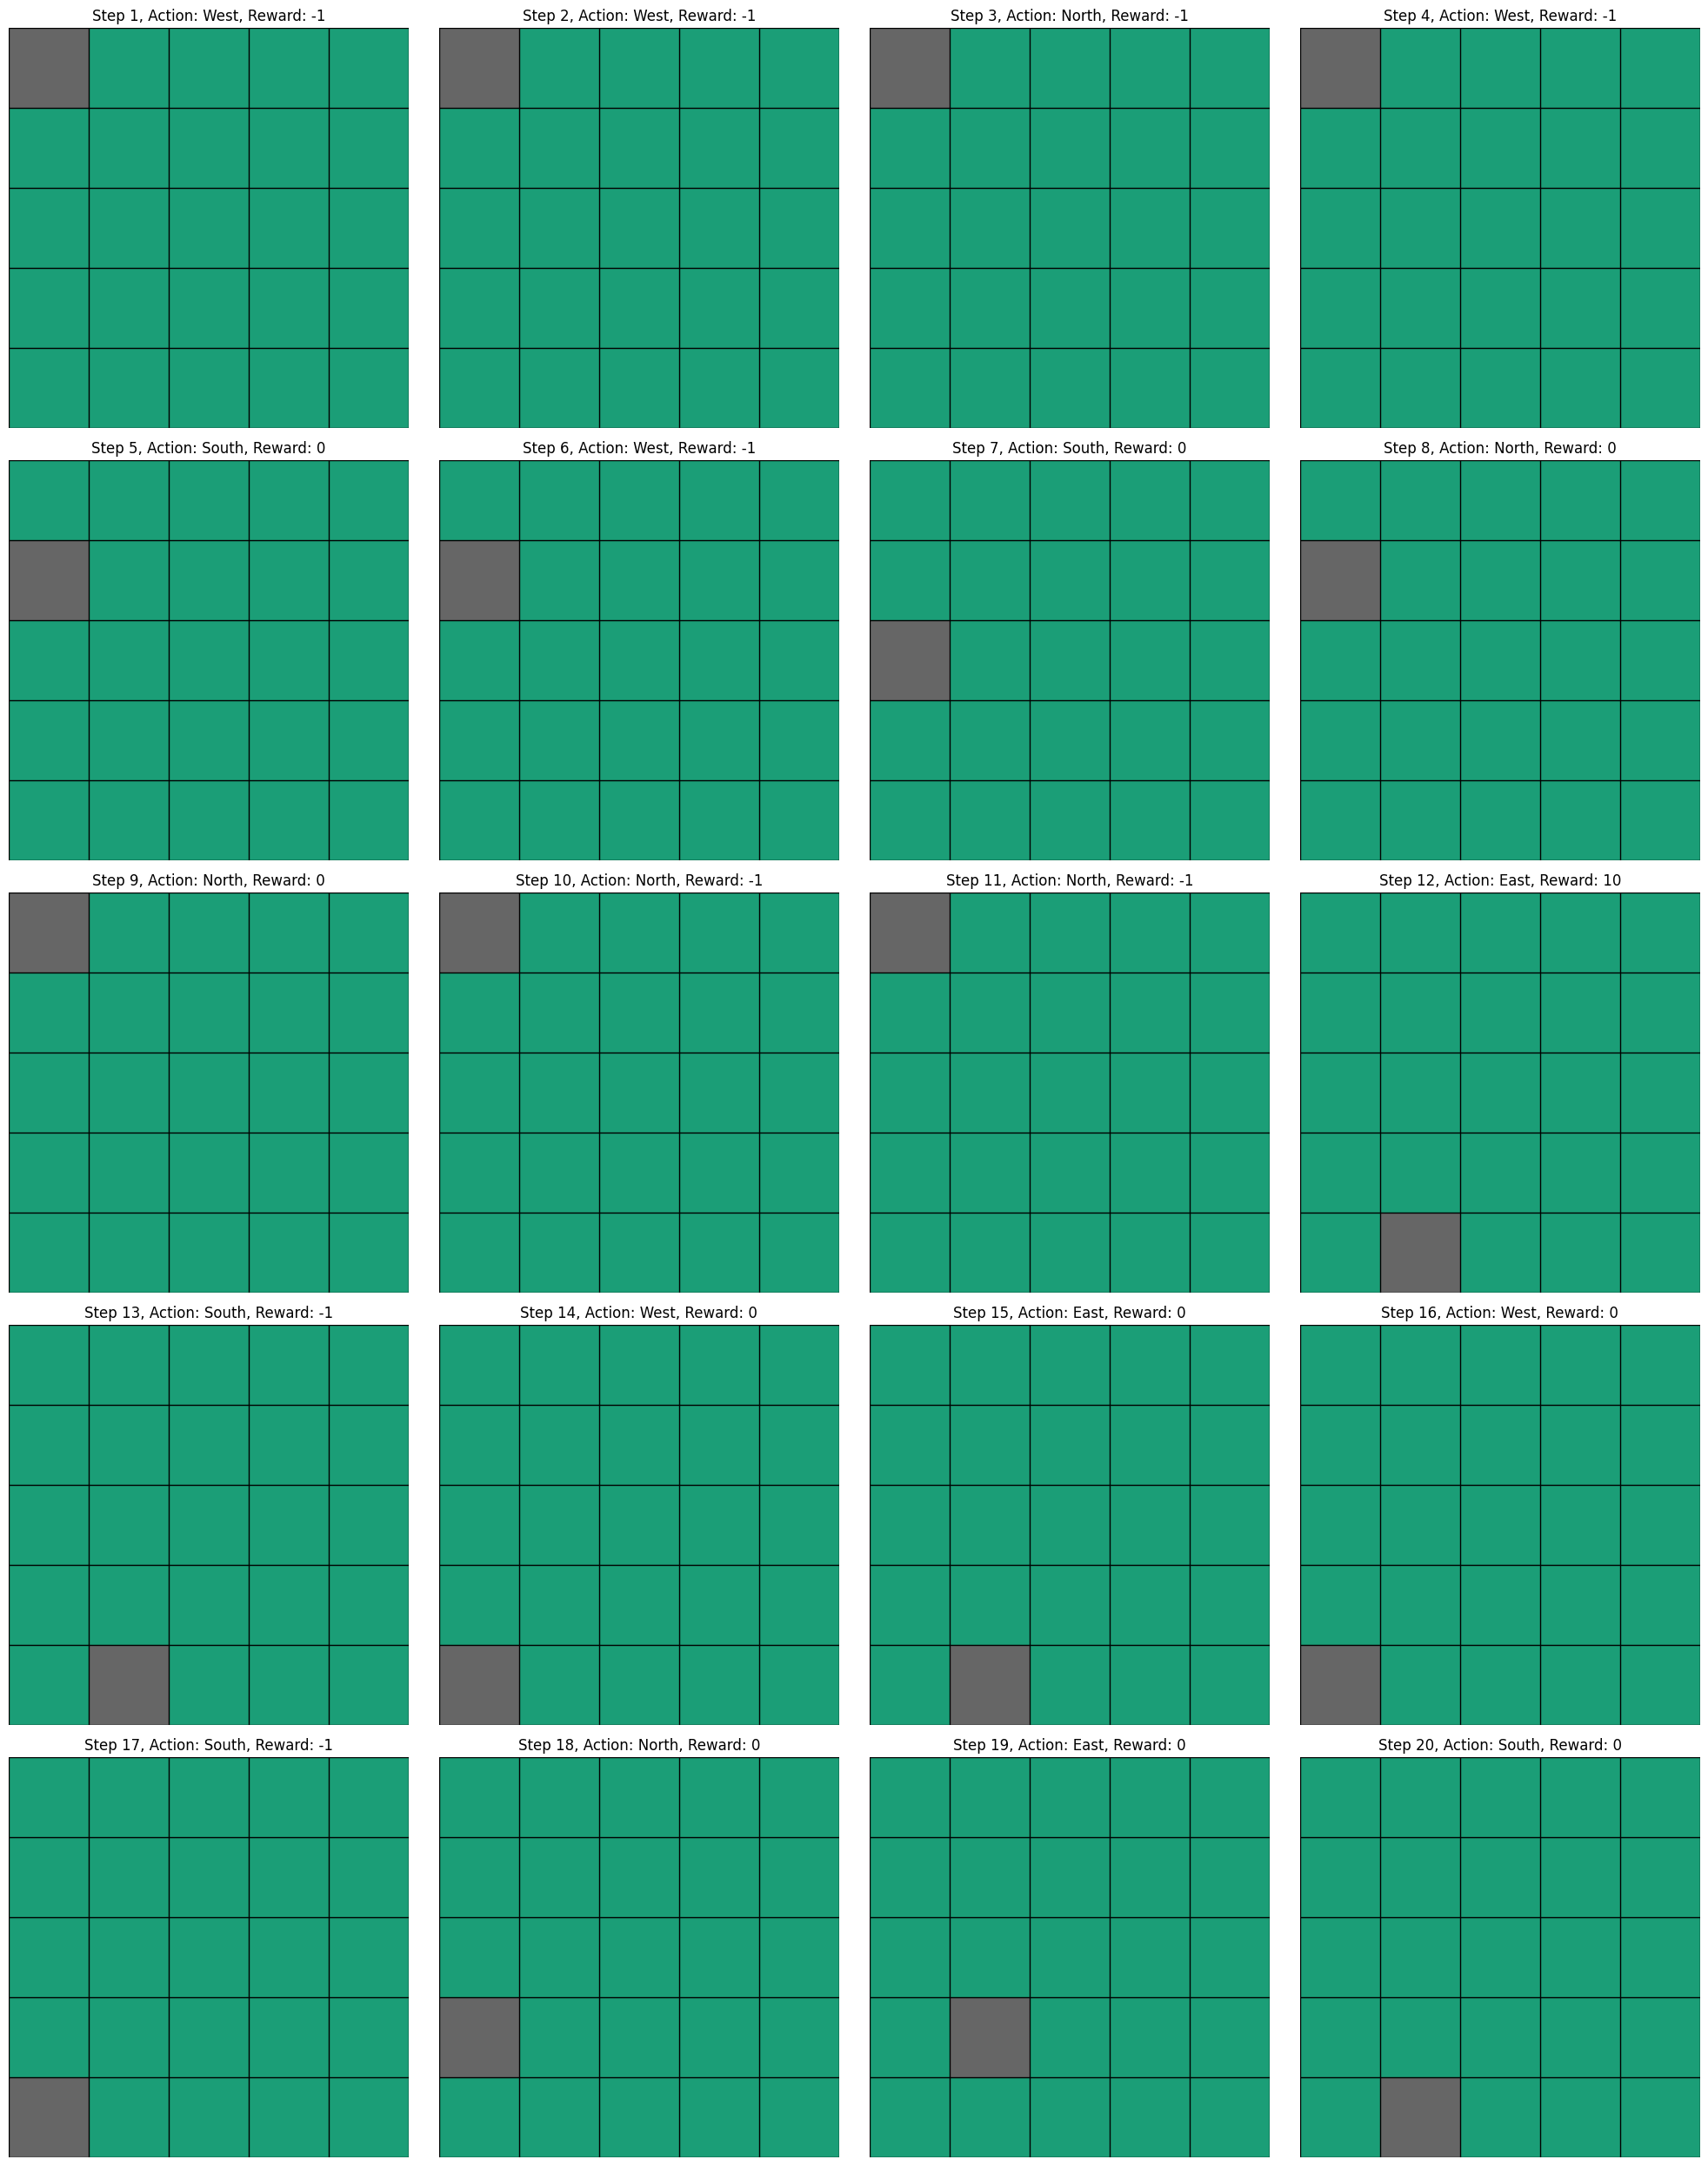
\includegraphics[width=0.9\textwidth]{images/20_steps.png}
		\caption{20 successive steps of the environment}
		\label{fig:1.1.a.1}
	\end{figure}
	
	\end{document}